\begin{frame}{El sonido}
  \begin{center}
    El \textbf{sonido} es una vibración en forma de onda.

    \bigskip
    \bigskip

    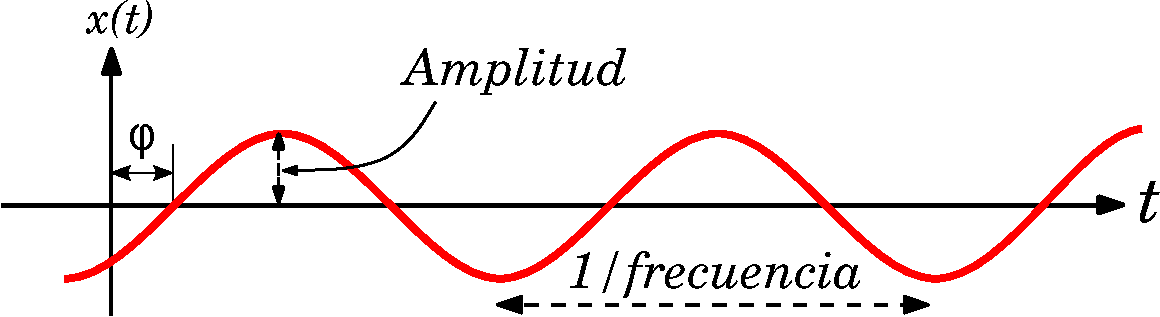
\includegraphics[width=0.8\textwidth]{imagenes/imagen_onda}

    \bigskip

    \begin{description}
    \item[Frecuencia] Oscilaciones por unidad de tiempo. 
    \item[Amplitud] Energía que transporta la onda.
    \item[Fase] Desplazamiento respecto del origen.
    \end{description}
  \end{center}
\end{frame}

\begin{frame}{Descomposición de sonidos}
  \begin{center}
    Los sonidos no suelen ser ondas puras, \\se componen de \textbf{parciales}.

    \pause \bigskip
  
    La \textbf{frecuencia fundamental} es el menor de esos parciales. Dicta la
    \textbf{altura} general del sonido.

    \pause \bigskip

    Los \textbf{armónicos} son parciales múltiplos de la frecuencia fundamental,
    enriquecen el sonido.

    \pause \bigskip
  
    {\large
    \textcolor{red}{\textbf{Objetivo:}} Descomponer el sonido para obtener la \\
    \textbf{frecuencia fundamental}.}
  \end{center}
\end{frame}

\begin{frame}{Herramientas de análisis armónico}
  \begin{center}
    Trabajan en el \textbf{dominio de la frecuencia}: se representa una señal
    respecto a su espectro de frecuencias.

    \pause \bigskip

    La \textbf{transformada de Fourier} es la herramienta más conocida:
    descompone una señal en sus componentes senoidales.

    \pause \bigskip

    Algoritmo más habitual: \textbf{FFT - Fast Fourier Transform}. \\En nuestro
    caso usamos la versión discreta, \\\textbf{DFT - Discrete Fourier Transform}.

  \end{center}
\end{frame}

\begin{frame}{Ejemplo de aplicación de FFT}
  \begin{center}
    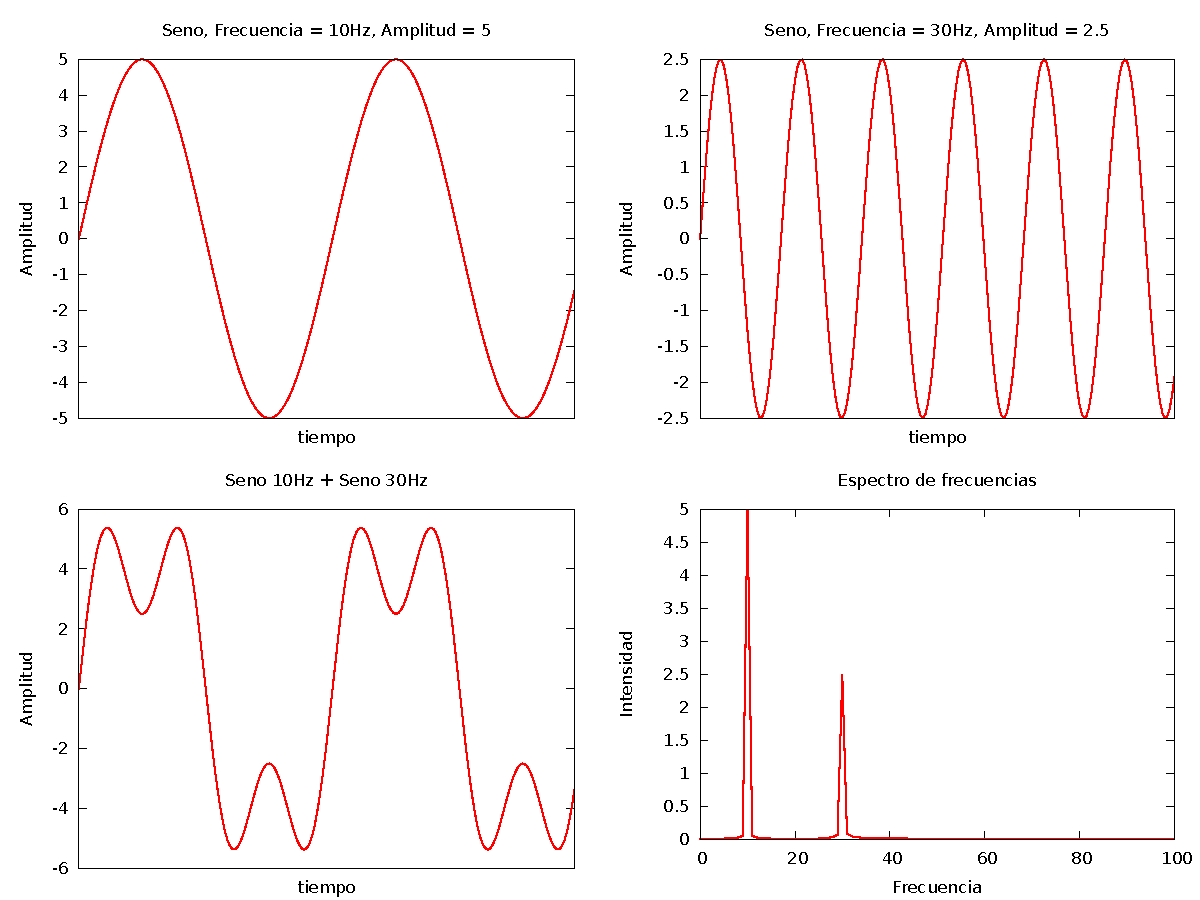
\includegraphics[width=\textwidth]{scripts_octave/imagen_senosEspectro}
  \end{center}
\end{frame}


%%% Local Variables: 
%%% mode: latex
%%% TeX-master: "../presentacion"
%%% End: 
